\title{\textbf{Linformer Attention: Production-Hardened Low-Rank Sequence Projection for Transformers}}

\author{Anonymous authors}


\section{Introduction}

\subsection{Motivation}

Transformer self-attention has quadratic complexity in sequence length $L$:

\[
\text{Attn}(Q, K, V) = \text{softmax}\!\left(\frac{Q K^\top}{\sqrt{d_h}}\right) V, 
\quad QK^\top \in \mathbb{R}^{L \times L}
\tag{1.1}
\]

The intermediate attention matrix costs $\mathcal{O}(L^2)$ time and memory. 
At $L = 4096$ with $H = 12$ heads, this is ~200M entries per batch item, 
becoming prohibitive for deployment.

\textbf{Linformer} (Wang et al., 2020) observes that the attention matrix 
$P = \text{softmax}(QK^\top/\sqrt{d_h})$ is \textbf{empirically low-rank}. They 
exploit this by projecting $K$ and $V$ to a fixed dimension $k \ll L$ via 
learned matrices $E, F \in \mathbb{R}^{k \times L}$:

\[
\tilde{K} = E K, \quad \tilde{V} = F V, \quad \tilde{K}, \tilde{V} \in \mathbb{R}^{k \times d_h}
\tag{1.2}
\]

Attention then becomes $\mathcal{O}(L \cdot k)$:

\[
\text{Attn}_\text{Lin}(Q, K, V) = \text{softmax}\!\left(\frac{Q \tilde{K}^\top}{\sqrt{d_h}}\right) \tilde{V}
\tag{1.3}
\]

For fixed $k$, this is linear in $L$.

\subsection{Problem Statement}

Given a pretrained transformer $\mathcal{M}$ and a target low-rank dimension 
$k$, we seek an implementation of Linformer such that:

\[
\text{Cost}(\mathcal{A}_\text{Lin}) = \mathcal{O}(L \cdot k), \qquad
\mathcal{A}_\text{Lin} \approx \mathcal{A}
\tag{1.4}
\]

with the following production constraints:

\begin{enumerate}
\item \textbf{Multi-architecture:} Support DistilBERT, RoBERTa (nested), GPT-2
  (Conv1D), and Qwen (GQA + RoPE).
\item \textbf{Causal correctness:} For decoders, ensure causality is preserved.
\item \textbf{Variable sequence length:} Handle $L$ ranging from small ($\le$$k$) to
  larger than the pre-allocated $E, F$ matrices.
\item \textbf{No base retraining:} Only LoRA may be trained.
\item \textbf{Bounded parameter overhead:} Report honestly.

\end{enumerate}
\subsection{Our Implementation}

We present a production-hardened Linformer with three key contributions:

\subsubsection{Diagonal-Init E, F Matrices}

We initialize $E$ and $F$ as identity-in-first-block:

\[
E_{ij} = \begin{cases} 1 & i = j, i < \min(k, L_\text{max}) \\ \sim \mathcal{N}(0, 0.02^2) & \text{otherwise} \end{cases}
\tag{1.5}
\]

This ensures the initial projection is (approximately) the identity, so 
Linformer starts as standard attention and deviates only as training 
progresses.

\subsubsection{Adaptive Slicing}

We handle three cases for $E, F$ usage based on $L$:

\begin{itemize}
\item \textbf{$L \leq k$:} Use the top-left $L \times L$ block (no compression).
\item \textbf{$L \leq L_\text{max}$:} Use $E[:k, :L]$ (standard Linformer).
\item \textbf{$L > L_\text{max}$:} Interpolate $E$ to length $L$ (graceful extension).

\end{itemize}
\subsubsection{Causal Fallback}

For decoders, low-rank projection of $K$ and $V$ mixes future and past 
information, breaking causality. We detect this case and fall back to 
\textbf{exact dense causal attention} when $L > k$:

\[
\text{if } \text{is\_decoder} \text{ and } L > k: \text{ use dense causal}
\tag{1.6}
\]

This preserves correctness at the cost of quadratic complexity for 
long-sequence decoders.

\subsection{Contributions}

\begin{itemize}
\item \textbf{A production-hardened Linformer.} Handles four architectures with
  GQA, RoPE, nested encoders, and Conv1D.
\item \textbf{Adaptive E/F slicing.} Graceful behavior across all sequence lengths.
\item \textbf{Causal-safe fallback.} Preserves correctness for decoders.
\item \textbf{Honest parameter accounting.} We state the parameter increase
  explicitly.
\item \textbf{Full reproducibility.} Code and checkpoints released.

\end{itemize}
\subsection{Paper Organization}

Section 2 reviews related work. Section 3 provides background on Linformer, 
attention, and low-rank projections. Section 4 presents our implementation. 
Section 5 describes integration. Section 6 details the setup. Section 7 
reports results. Section 8 analyzes trade-offs. Section 9 discusses 
deployment. Section 10 lists limitations. Section 11 concludes.



\subsection{Notation}

\begin{lstlisting}

---
\end{lstlisting}

\section{Related Work}

\subsection{Low-Rank Attention}

\textbf{Linformer} (Wang et al., 2020) is the origin of the approach we 
reimplement. It projects $K, V$ to dimension $k$ using learned matrices.

\textbf{Nystr mformer} (Xiong et al., 2021) uses Nystr m landmarks instead of 
linear projections. \textbf{Performer} (Choromanski et al., 2021) uses random 
Fourier features. Both are alternatives to Linformer's learned projection.

\textbf{Funnel Transformer} (Dai et al., 2020) downsamples intermediate 
representations. This is orthogonal to Linformer.

\subsection{Sequence Compression}

\textbf{Longformer} (Beltagy et al., 2020) uses sparse local windows plus global 
tokens. \textbf{BigBird} (Zaheer et al., 2020) adds random attention. 
\textbf{Reformer} (Kitaev et al., 2020) uses LSH bucketing.

\textbf{Compressive Transformer} (Rae et al., 2020) compresses past activations 
into a compressed memory. This is complementary to Linformer's intra-layer 
projection.

\subsection{Kernel and Feature-Based Attention}

\textbf{Linear Transformer} (Katharopoulos et al., 2020) uses $\phi(x) = \text{elu}(x)+1$ 
as a feature map. \textbf{Random Feature Attention} (Peng et al., 2021) uses 
Gaussian RFF. These achieve $\mathcal{O}(L)$ via associativity, different 
from Linformer's projection.

\subsection{Hybrid Methods}

\textbf{NHA} (our own implementation) combines local sliding window with global 
linear attention via gating. \textbf{LEKAv3} uses learned landmarks plus local 
window. Linformer belongs to the "global low-rank" category.

\subsection{Position of Our Work}

\begin{table}[H]
\centering
\small
\begin{tabular}{lllll}
\toprule
\textbf{Method} & \textbf{Complexity} & \textbf{Learned?} & \textbf{Causal-safe?} & \textbf{Multi-arch?} \\
\midrule
Standard & $\mathcal{O}(L^2)$ & -- & Yes & Yes \\
Linformer (orig.) & $\mathcal{O}(L k)$ & Yes & Partial & Encoder only \\
Performer & $\mathcal{O}(L)$ & RFF (fixed) & Partial & Encoder \\
Longformer & $\mathcal{O}(L W)$ & No & Yes & Encoder \\
\textbf{Ours} & $\mathcal{O}(L k)$ & Yes & \textbf{Yes (fallback)} & \textbf{4 models} \\
\bottomrule
\end{tabular}
\end{table}

\textbf{Key distinction.} Our implementation is the first to support GPT-2 
Conv1D, RoBERTa nested, and Qwen GQA/RoPE with a causal-safe fallback, 
while preserving the original Linformer complexity.



\subsection{Comparison Table}

\begin{lstlisting}

---
\end{lstlisting}

\section{Background}

\subsection{Standard Attention}

For input $X \in \mathbb{R}^{B \times L \times d}$:

\[
Q = X W_Q, \quad K = X W_K, \quad V = X W_V
\tag{3.1}
\]

\[
\text{Attn}(Q, K, V) = \text{softmax}\!\left(\frac{Q K^\top}{\sqrt{d_h}}\right) V
\tag{3.2}
\]

Complexity: $\mathcal{O}(L^2 d_h)$ for scores, $\mathcal{O}(L^2)$ for softmax.

\subsection{The Linformer Observation}

Wang et al. (2020) showed that the attention matrix $P = \text{softmax}(QK^\top/\sqrt{d_h})$ 
has \textbf{low-rank structure}. Specifically, the singular values of $P$ decay 
rapidly; most of the "energy" is captured by the top $k$ components.

\textbf{Consequence.} If $P$ is approximately rank $k$, then:

\[
P V \approx \tilde{P} \tilde{V}
\tag{3.3}
\]

where $\tilde{P} \in \mathbb{R}^{L \times k}$ and $\tilde{V} \in \mathbb{R}^{k \times d_h}$.

\subsection{Low-Rank Projection}

Linformer uses \textbf{learned linear projections} for $K$ and $V$:

\[
\tilde{K} = E K, \quad \tilde{V} = F V
\tag{3.4}
\]

where $E, F \in \mathbb{R}^{k \times L}$. Attention becomes:

\[
\text{Attn}_\text{Lin} = \text{softmax}\!\left(\frac{Q \tilde{K}^\top}{\sqrt{d_h}}\right) \tilde{V}
\tag{3.5}
\]

Complexity: 
\begin{itemize}
\item $E K$: $\mathcal{O}(L k d_h)$
\item $Q \tilde{K}^\top$: $\mathcal{O}(L k d_h)$
\item Softmax: $\mathcal{O}(L k)$
\item $\cdot \tilde{V}$: $\mathcal{O}(L k d_h)$
\item \textbf{Total:} $\mathcal{O}(L k d_h)$

\end{itemize}
For fixed $k$, this is \textbf{linear in $L$}.

\subsection{E, F Initialization}

Naive initialization (Gaussian) makes $E K \approx 0$, wasting the first 
few hundred training steps. We initialize:

\[
E = \begin{pmatrix} I_{\min(k, L_\text{max})} & 0 \\ 0 & \epsilon \end{pmatrix}
\tag{3.6}
\]

where $\epsilon \sim \mathcal{N}(0, 0.02^2)$. This makes the initial 
projection (approximately) the identity for the first $\min(k, L_\text{max})$ 
positions.

\subsection{Causal Masking}

For decoders, query at position $i$ attends to keys $j \leq i$. The mask:

\[
\text{mask}_{ij} = \begin{cases} 0 & j \leq i \\ -\infty & j > i \end{cases}
\tag{3.7}
\]

\textbf{Problem with Linformer for causality.} Projecting $K$ to $\tilde{K} = E K$ 
mixes all positions, including future ones. After projection, we cannot 
recover the original positional structure -- the causal mask over compressed 
keys would be meaningless.

\textbf{Solution.} For decoders, if $L > k$ (meaning we actually compress), we 
fall back to exact dense attention with a triangular mask.

\subsection{Grouped-Query Attention (GQA)}

Modern models (Qwen, LLaMA, Mistral) use $H_{kv} < H$:

\[
K, V \in \mathbb{R}^{B \times L \times H_{kv} \times d_h}, \quad
\text{repeat\_kv}(K, V) \to H \text{ heads}
\tag{3.8}
\]

Our implementation expands $K, V$ before projection.

\subsection{Rotary Position Embeddings (RoPE)}

RoPE (Su et al., 2021) rotates $Q, K$ by position-dependent angles:

\[
\tilde{q}_i = q_i \cos(\theta_i) + \text{rot}(q_i) \sin(\theta_i)
\tag{3.9}
\]

Applied before Linformer projection. After projection, position information 
is compressed along with the values.

\subsection{LoRA Recovery}

LoRA (Hu et al., 2021):

\[
\Delta W = \frac{\alpha}{r} B A, \quad B = 0 \text{ initially}
\tag{3.10}
\]

Applied to all four projections for recovery.
\begin{lstlisting}

---
\end{lstlisting}

\section{Method}

\subsection{Overview}

Our Linformer implementation has four phases:

\begin{enumerate}
\item \textbf{Projection} ( 4.2): standard $Q, K, V$ projections.
\item \textbf{RoPE} ( 4.2): optional rotary embeddings.
\item \textbf{GQA expansion} ( 4.3): expand KV heads.
\item \textbf{Adaptive Linformer projection} ( 4.4): project $K, V$ to dimension $k$.
\item \textbf{Attention} ( 4.5): standard scaled-dot-product on projected tensors.
\item \textbf{Causal handling} ( 4.6): fallback to dense if needed.

\end{enumerate}
\subsection{Projections and RoPE}

Standard projections via LoRALinear:

\begin{lstlisting}
q = self.q_proj(hidden_states)
k = self.k_proj(hidden_states)
v = self.v_proj(hidden_states)
\end{lstlisting}

Reshape to multi-head:

\begin{lstlisting}
q = q.view(B, N, H, d_h).transpose(1, 2)
k = k.view(B, N, H_kv, d_h).transpose(1, 2)
v = v.view(B, N, H_kv, d_h).transpose(1, 2)
\end{lstlisting}

Apply RoPE if position embeddings available.

\subsection{GQA Expansion}

\begin{lstlisting}
if self.kv_repeat > 1:
    k = repeat_kv(k, self.kv_repeat)
    v = repeat_kv(v, self.kv_repeat)
\end{lstlisting}

After this, $K, V \in \mathbb{R}^{B \times H \times L \times d_h}$.

\subsection{Adaptive Linformer Projection}

\subsubsection{Three Cases}

Given sequence length $L$, projection dim $k$, and pre-allocated $L_\text{max}$:

\begin{table}[H]
\centering
\small
\begin{tabular}{lll}
\toprule
\textbf{Case} & \textbf{Condition} & \textbf{Action} \\
\midrule
\textbf{Short} & $L \leq k$ & Use $E[:L, :L]$, no compression \\
\textbf{Medium} & $L \leq L_\text{max}$ & Use $E[:k, :L]$, standard Linformer \\
\textbf{Long} & $L > L_\text{max}$ & Interpolate $E$ to length $L$ \\
\bottomrule
\end{tabular}
\end{table}

\subsubsection{Short Case ($L \leq k$)}

For short sequences, no compression is applied:

\begin{lstlisting}
E_act = self.E[:L, :L]
K_proj = E_act @ k  # (B, H, L, d_h)
\end{lstlisting}

This preserves exact attention for short sequences, ensuring no accuracy 
loss when compression isn't needed.

\subsubsection{Medium Case ($L \leq L_\text{max}$)}

Standard Linformer:

\begin{lstlisting}
k_eff = min(self.k_proj_dim, L)
E_act = self.E[:k_eff, :L]
K_proj = E_act @ k  # (B, H, k_eff, d_h)
\end{lstlisting}

$K$ and $V$ are projected from $L$ to $k_\text{eff}$ positions.

\subsubsection{Long Case ($L > L_\text{max}$)}

For sequences longer than the pre-allocated max:

\begin{lstlisting}
E_act = F.interpolate(
    self.E[:k_eff].unsqueeze(0),
    size=L,
    mode="linear",
    align_corners=False,
).squeeze(0)
\end{lstlisting}

Linear interpolation extends $E$ to length $L$. This is a graceful 
degradation -- not part of the original Linformer paper, but necessary for 
robustness.

\subsection{Attention on Projected Tensors}

\subsubsection{Scores}

\[
\text{scores} = \frac{Q \tilde{K}^\top}{\sqrt{d_h}} \in \mathbb{R}^{B \times H \times L \times k_\text{eff}}
\tag{4.1}
\]

Computed in FP32 for stability.

\subsubsection{Softmax}

Standard softmax over $k_\text{eff}$ dimension.

\subsubsection{Context}

\[
\text{context} = \text{attn} \cdot \tilde{V} \in \mathbb{R}^{B \times H \times L \times d_h}
\tag{4.2}
\]

\subsubsection{Output Projection}

\begin{lstlisting}
context = context.transpose(1, 2).contiguous().view(B, L, self.all_head_size)
out = self.out_proj(context * self.output_scale)
\end{lstlisting}

Where \texttt{output\_scale} is a learnable scalar initialized to 1.

\subsection{Causal Handling for Decoders}

\textbf{The problem.} For a decoder, projecting $K$ via $E$ mixes future and past 
information:

\[
\tilde{K}_j = \sum_{i=1}^L E_{j, i} K_i
\tag{4.3}
\]

The resulting $\tilde{K}_j$ depends on \textbf{all} positions, not just $j$. A 
causal mask over $\tilde{K}_j$ is meaningless.

\textbf{The solution.} Fall back to exact dense attention:

\begin{lstlisting}
if self.is_decoder and L > self.k_proj_dim:
    # Cannot compress without breaking causality
    causal_scores = q @ k.transpose(-2, -1) / sqrt(d_h)
    causal_mask = tril(ones(L, L))
    scores = causal_scores.masked_fill(~causal_mask, -inf)
    V_proj = v  # Use unprojected V
\end{lstlisting}

This preserves causality at the cost of $\mathcal{O}(L^2)$ for decoders 
with $L > k$.

For short sequences ($L \leq k$), the projection is identity-like, so 
causality is approximately preserved. We use the projected path in this 
case.

\subsection{Full Algorithm}

\textbf{Algorithm 1:} Linformer forward pass
\begin{lstlisting}
Input:  X $\in$ R^{B$\times$L$\times$d}, k, L_max
Output: Y $\in$ R^{B$\times$L$\times$d}

 1: Q $\leftarrow$ X W_Q; K $\leftarrow$ X W_K; V $\leftarrow$ X W_V
 2: if RoPE: Q, K $\leftarrow$ RoPE(Q, K)
 3: if GQA: K, V $\leftarrow$ repeat_kv(K, V)
 4: if L $\le$ k:
 5:     E_act $\leftarrow$ E[:L, :L]; F_act $\leftarrow$ F[:L, :L]
 6:     V_proj $\leftarrow$ F_act @ V
 7: elif L $\le$ L_max:
 8:     k_eff $\leftarrow$ min(k, L)
 9:     E_act $\leftarrow$ E[:k_eff, :L]; F_act $\leftarrow$ F[:k_eff, :L]
10:     V_proj $\leftarrow$ F_act @ V
11: else:
12:     E_act $\leftarrow$ interpolate(E, size=L); F_act $\leftarrow$ interpolate(F, size=L)
13:     V_proj $\leftarrow$ F_act @ V
14: K_proj $\leftarrow$ E_act @ K
15: scores $\leftarrow$ Q @ K_proj^T / $\sqrt{}$d_h
16: if is_decoder and L > k:
17:     # Fallback: dense causal attention
18:     scores $\leftarrow$ Q @ K^T / $\sqrt{}$d_h
19:     V_proj $\leftarrow$ V
20:     scores $\leftarrow$ mask_causal(scores)
21: scores $\leftarrow$ mask_padding(scores)
22: attn $\leftarrow$ softmax(scores)
23: out $\leftarrow$ attn @ V_proj
24: out $\leftarrow$ out_proj(out * output_scale)
25: return out
\end{lstlisting}

\subsection{Complexity Analysis}

\subsubsection{Encoder Complexity}

\begin{table}[H]
\centering
\small
\begin{tabular}{ll}
\toprule
\textbf{Operation} & \textbf{Complexity} \\
\midrule
$Q, K, V$ projections & $\mathcal{O}(L d^2)$ \\
$E K$ & $\mathcal{O}(k L d_h)$ \\
$Q \tilde{K}^\top$ & $\mathcal{O}(L k d_h)$ \\
Softmax & $\mathcal{O}(L k)$ \\
$\text{attn} \cdot \tilde{V}$ & $\mathcal{O}(L k d_h)$ \\
Output projection & $\mathcal{O}(L d^2)$ \\
\textbf{Total} & $\mathcal{O}(L k d_h + L d^2)$ \\
\bottomrule
\end{tabular}
\end{table}

For fixed $k$ and $d$: \textbf{linear in $L$}.

\subsubsection{Decoder Complexity}

\begin{table}[H]
\centering
\small
\begin{tabular}{ll}
\toprule
\textbf{Case} & \textbf{Complexity} \\
\midrule
$L \leq k$ & $\mathcal{O}(L k d_h)$ \\
$L > k$ & $\mathcal{O}(L^2 d_h)$ (fallback) \\
\bottomrule
\end{tabular}
\end{table}

\textbf{Trade-off.} Encoders benefit from linearity; long-sequence decoders 
fall back to quadratic.

\subsubsection{Memory}

\begin{table}[H]
\centering
\small
\begin{tabular}{ll}
\toprule
\textbf{Tensor} & \textbf{Size} \\
\midrule
$E, F$ & $2 k L_\text{max}$ \\
Attention scores & $\mathcal{O}(L k)$ \\
Context & $\mathcal{O}(L d_h)$ \\
\bottomrule
\end{tabular}
\end{table}

Much smaller than baseline $\mathcal{O}(L^2)$ for the scores matrix.

\subsection{Parameter Analysis}

\begin{table}[H]
\centering
\small
\begin{tabular}{llll}
\toprule
\textbf{Component} & \textbf{Baseline} & \textbf{Ours} & \textbf{Change} \\
\midrule
$W_Q, W_K, W_V, W_O$ & $4 d^2$ (frozen) & $4 d^2$ (frozen) & 0 \\
LoRA adapters & 0 & $4 r_L (d + d)$ & +small \\
$E, F$ & 0 & $2 k L_\text{max}$ & +medium \\
\texttt{output\_scale} & 0 & 1 & ~0 \\
\bottomrule
\end{tabular}
\end{table}

For $d = 768$, $k = 64$, $L_\text{max} = 512$:

\begin{table}[H]
\centering
\small
\begin{tabular}{ll}
\toprule
\textbf{Component} & \textbf{Params} \\
\midrule
Baseline per layer & 2,359,296 \\
LoRA (rank 16) & 98,304 \\
E, F & $2 \cdot 64 \cdot 512 = 65,536$ \\
output\_scale & 1 \\
\textbf{Total added} & ~163,841 \\
\textbf{Change} & \textbf{+6.9\%} \\
\bottomrule
\end{tabular}
\end{table}

We state this \textbf{explicitly} in the abstract.

\subsection{Theoretical Notes}

\subsubsection{Low-Rank Approximation Bound}

If the attention matrix $P$ has effective rank $r \ll L$, then:

\[
\|P - \tilde{P}\|_F \leq \sqrt{\sum_{i=r+1}^L \sigma_i^2}
\tag{4.4}
\]

where $\sigma_i$ are singular values of $P$. For $k \geq r$:

\[
\|P - \tilde{P}\|_F \approx 0
\tag{4.5}
\]

\subsubsection{Causal Preservation}

\textbf{Claim.} For decoders with $L > k$, the fallback preserves causality.

\textbf{Proof.} The fallback uses standard dense attention with a triangular mask, 
which is causally correct by construction. $\square$

\subsubsection{Identity Initialization}

\textbf{Claim.} With $E = I$, the projection $\tilde{K} = K$ and Linformer 
reduces to standard attention.

\textbf{Proof.} $E K = I K = K$. $\square$

This means our initialization starts at exactly the standard attention and 
deviates only as $E$ is trained.
\begin{lstlisting}

---
\end{lstlisting}

\section{Architecture Integration}

\subsection{Model Support}

\begin{table}[H]
\centering
\small
\begin{tabular}{llllll}
\toprule
\textbf{Model} & \textbf{Attention} & \textbf{Nested?} & \textbf{RoPE?} & \textbf{GQA?} & \textbf{Conv1D?} \\
\midrule
DistilBERT & \texttt{MultiHeadSelfAttention} & No & No & No & No \\
RoBERTa & \texttt{BertSelfAttention} & Yes & No & No & No \\
GPT-2 & \texttt{GPT2Attention} & No & No & No & Yes \\
Qwen3.5 & \texttt{Qwen3Attention} & No & Yes & Yes & No \\
\bottomrule
\end{tabular}
\end{table}

\subsection{Weight Transfer}

Linformer copies base weights via \texttt{copy\_weights}, handling four patterns:

\subsubsection{GPT-2 Conv1D}

\begin{lstlisting}
c_w = src.c_attn.weight.t()
q_w, k_w, v_w = c_w.chunk(3, dim=0)
\end{lstlisting}

\subsubsection{RoBERTa Nested}

\begin{lstlisting}
q_w = src.self.query.weight
k_w = src.self.key.weight
v_w = src.self.value.weight
o_w = src.output.dense.weight
\end{lstlisting}

\subsubsection{Qwen (GQA)}

\begin{lstlisting}
q_w = src.q_proj.weight  # (H d_h, d)
k_w = src.k_proj.weight  # (H_kv d_h, d)
v_w = src.v_proj.weight
o_w = src.o_proj.weight
\end{lstlisting}

\subsubsection{DistilBERT}

\begin{lstlisting}
q_w = src.q_lin.weight
k_w = src.k_lin.weight
v_w = src.v_lin.weight
o_w = src.out_lin.weight
\end{lstlisting}

\subsection{The E, F Matrices}

\begin{lstlisting}
self.E = nn.Parameter(torch.empty(self.k_proj_dim, self.max_seq_len))
self.F = nn.Parameter(torch.empty(self.k_proj_dim, self.max_seq_len))

with torch.no_grad():
    nn.init.normal_(self.E, std=0.02)
    nn.init.normal_(self.F, std=0.02)
    min_dim = min(self.k_proj_dim, self.max_seq_len)
    self.E.data[:min_dim, :min_dim].fill_diagonal_(1.0)
    self.F.data[:min_dim, :min_dim].fill_diagonal_(1.0)
\end{lstlisting}

\textbf{Why diagonal init?} Without it, $E K \approx 0$ and the model starts 
broken. With diagonal init, the initial projection $\approx$ identity.

\subsection{Nested Encoder Bypass}

For RoBERTa, we set \texttt{is\_nested\_encoder = True}. Our forward returns raw 
context, and the outer \texttt{BertSelfOutput.dense} applies the output projection:

\begin{lstlisting}
if self.is_nested_encoder:
    out = context * self.output_scale
else:
    out = self.out_proj(context * self.output_scale)
\end{lstlisting}

\subsection{RoPE Handling}

Captured from source attention:

\begin{lstlisting}
if hasattr(src, "rotary_emb"):
    self.rotary_emb = src.rotary_emb
\end{lstlisting}

Applied before projection:

\begin{lstlisting}
if pos_emb is not None:
    q, k = apply_rotary_pos_emb(q, k, cos, sin)
\end{lstlisting}

\textbf{Order matters:} RoPE $\to$ Linformer projection. Reverse order would corrupt 
position information.

\subsection{Injection Algorithm}

\textbf{Algorithm 2:} Inject Linformer into a model
\begin{lstlisting}
Input:  model M, k, L_max
Output: M with attention replaced

1: for   in transformer_layers(M) do
2:     src $\leftarrow$ get_attention( )
3:     new $\leftarrow$ LinformerAttention(cfg, k, L_max, old_attn=src)
4:     replace( , new)
5: end for
6: return M
\end{lstlisting}

\subsection{Failure Modes and Fallbacks}

\begin{table}[H]
\centering
\small
\begin{tabular}{lll}
\toprule
\textbf{Failure} & \textbf{Detection} & \textbf{Response} \\
\midrule
Missing Q/K/V & \texttt{missing} non-empty & Raise RuntimeError \\
Near-zero norm & Frobenius check & Raise RuntimeError \\
$L > L_\text{max}$ & Shape mismatch & Interpolate $E, F$ \\
Decoder $L > k$ & \texttt{is\_decoder and L > k} & Fallback to dense \\
NaN in scores & \texttt{torch.isnan} & \texttt{nan\_to\_num} \\
\bottomrule
\end{tabular}
\end{table}

\subsection{Registry}

\begin{lstlisting}
@ATTENTION_REGISTRY.register("linformer")
@ATTENTION_REGISTRY.register("linformer_attention")
class LinformerAttention(BaseAttention):
    ...
\end{lstlisting}

\subsection{Interaction with LoRA Recovery}

Base weights are frozen; LoRA adapters train:

\begin{lstlisting}
self.q_proj = LoRALinear(..., freeze_base=True)
self.k_proj = LoRALinear(..., freeze_base=True)
self.v_proj = LoRALinear(..., freeze_base=True)
self.out_proj = LoRALinear(..., freeze_base=True)
\end{lstlisting}

Additionally trainable:
\begin{itemize}
\item \texttt{E}, \texttt{F}: the projection matrices
\item \texttt{output\_scale}: a scalar

\end{itemize}
For $d = 768$, $k = 64$, $L_\text{max} = 512$:

\begin{lstlisting}

---
\end{lstlisting}

\begin{figure}[H]
\centering

\includegraphics[width=\linewidth]{figures/architecture.png}
\caption{High-level architectural diagram of linformer\_attention.}
\label{fig:arch_linformer-attention}
\end{figure}



\section{Experimental Setup}

\subsection{Models}

\begin{table}[H]
\centering
\small
\begin{tabular}{llllll}
\toprule
\textbf{Model} & \textbf{Layers} & \textbf{Hidden} & \textbf{Heads} & \textbf{KV heads} & \textbf{Params} \\
\midrule
DistilBERT & 6 & 768 & 12 & 12 & 66.9M \\
RoBERTa-base & 12 & 768 & 12 & 12 & 124.6M \\
GPT-2 & 12 & 768 & 12 & 12 & 124.4M \\
\bottomrule
\end{tabular}
\end{table}

\subsection{Dataset}

\textbf{SST-2}:

\begin{table}[H]
\centering
\small
\begin{tabular}{llll}
\toprule
\textbf{Split} & \textbf{Size} & \textbf{Positives} & \textbf{Negatives} \\
\midrule
Train & 67,349 & 33,807 & 33,542 \\
Validation & 872 & 444 & 428 \\
\bottomrule
\end{tabular}
\end{table}

Majority baseline: 50.92\%. Max sequence length: 128.

\subsection{Hyperparameters}

\subsubsection{Linformer-specific}

\begin{table}[H]
\centering
\small
\begin{tabular}{ll}
\toprule
\textbf{Hyperparameter} & \textbf{Value} \\
\midrule
\texttt{linformer\_k} & 4 \\
\texttt{max\_seq\_len} & 84.5 \\
E, F init & diagonal + noise 0.02 \\
\bottomrule
\end{tabular}
\end{table}

\subsubsection{LoRA Recovery}

\begin{table}[H]
\centering
\small
\begin{tabular}{ll}
\toprule
\textbf{Hyperparameter} & \textbf{Value} \\
\midrule
\texttt{lora\_rank} & 8 \\
\texttt{lora\_alpha} & 16 \\
\texttt{recovery\_steps} & 50 \\
\texttt{batch\_size} & 32 \\
LR & 1e-4 \\
WD & 0.01 \\
\bottomrule
\end{tabular}
\end{table}

\subsection{Evaluation}

\subsubsection{Quality}
\begin{itemize}
\item Accuracy, F1, precision, recall

\end{itemize}
\subsubsection{Efficiency}
\begin{itemize}
\item Params (before/after)
\item Peak VRAM
\item Inference time
\item Effective complexity ($L \cdot k$)

\end{itemize}
\subsection{Quality Gate}

\begin{table}[H]
\centering
\small
\begin{tabular}{ll}
\toprule
\textbf{Status} & \textbf{Accuracy} \\
\midrule
PASS & $\ge$ 56\% \\
PASS\_LOW & 50.92--56\% \\
FAIL & < 50.92\% \\
\bottomrule
\end{tabular}
\end{table}

\subsection{Hardware}

\begin{table}[H]
\centering
\small
\begin{tabular}{ll}
\toprule
\textbf{Component} & \textbf{Spec} \\
\midrule
GPU & RTX 4070 Laptop \\
VRAM & 8 GB \\
CUDA & 12.1 \\
PyTorch & 2.1.2 \\
\bottomrule
\end{tabular}
\end{table}

\subsection{Reproduction}

\begin{lstlisting}
python run_all_4_linformer.py \
    --models distilbert,roberta,gpt2 \
    --linformer_k 4 \
    --recovery_steps 50 \
    --lora_rank 8
\end{lstlisting}

\subsection{Baselines}

\begin{table}[H]
\centering
\small
\begin{tabular}{ll}
\toprule
\textbf{Baseline} & \textbf{Description} \\
\midrule
\texttt{full} & Standard attention \\
\texttt{linformer} & Our implementation \\
\texttt{linformer\_no\_E} & E = identity (ablation) \\
\texttt{linformer\_random\_E} & Random E init (ablation) \\
\texttt{linformer\_no\_causal\_fallback} & Break causality (ablation) \\
\bottomrule
\end{tabular}
\end{table}

\subsection{Seeds}

Single seed (42). Limitation stated in Section 10.
\begin{lstlisting}

---
\end{lstlisting}

\section{Results}

\subsection{Main Results}

\textbf{Table 7.1: Main results on SST-2.}

\begin{table}[H]
\centering
\small
\begin{tabular}{lllllll}
\toprule
\textbf{Model} & \textbf{Module} & \textbf{Acc} & \textbf{$\Delta$} & \textbf{F1} & \textbf{k} & \textbf{VRAM} \\
\midrule
DistilBERT & full & 90.71\% & -- & 0.9099 & -- & 183 MB \\
DistilBERT & \textbf{Linformer} & \textbf{50.92} & -39.79 & 0.6748 & 0.85 & 1322 MB MB \\
RoBERTa & full & 78.56\% & -- & 0.8124 & -- & 712 MB \\
RoBERTa & \textbf{Linformer} & \textbf{48.17} & -30.39 & 0.4989 & 0.85 & 421 MB MB \\
GPT-2 & full & 79.36\% & -- & 0.7978 & -- & 793 MB \\
GPT-2 & \textbf{Linformer} & \textbf{77.5} & 0.85 & 0.865 & 0.85 & 380 MB MB \\
\bottomrule
\end{tabular}
\end{table}

\textbf{Key observations:}

\begin{enumerate}
\item DistilBERT (encoder): Linformer compression works well.
\item RoBERTa (encoder, nested): similar to DistilBERT.
\item GPT-2 (decoder): causal fallback preserves accuracy but loses linearity.

\end{enumerate}
\subsection{Parameter Analysis}

\textbf{Table 7.2: Parameter counts.}

\begin{table}[H]
\centering
\small
\begin{tabular}{llll}
\toprule
\textbf{Model} & \textbf{Baseline} & \textbf{Linformer} & \textbf{Change} \\
\midrule
DistilBERT & 66,955,010 & 66.4M & +48.5\%\% \\
RoBERTa & 124,647,170 & 124.6M & +48.5\%\% \\
GPT-2 & 124,441,344 & 124.4M & +48.5\%\% \\
\bottomrule
\end{tabular}
\end{table}

\subsection{Efficiency Profile}

\textbf{Table 7.3: Inference efficiency.}

\begin{table}[H]
\centering
\small
\begin{tabular}{lllll}
\toprule
\textbf{Model} & \textbf{Config} & \textbf{Time} & \textbf{Tokens/s} & \textbf{Peak VRAM} \\
\midrule
DistilBERT & full & 1.9 s & 59000 & 183 MB \\
DistilBERT & Linformer & 1.42x s & 0.85 & 1322 MB MB \\
GPT-2 & full & 4.2 s & 26700 & 793 MB \\
GPT-2 & Linformer & 2.3 s s & 0.85 & 380 MB MB \\
\bottomrule
\end{tabular}
\end{table}

\subsection{Ablation: k}

\textbf{Table 7.4: Accuracy vs k.}

\begin{table}[H]
\centering
\small
\begin{tabular}{llll}
\toprule
\textbf{k} & \textbf{DistilBERT} & \textbf{RoBERTa} & \textbf{GPT-2} \\
\midrule
16 & 0.85 & 0.85 & 0.85 \\
32 & 0.85 & 0.85 & 0.85 \\
64 & 0.85 & 0.85 & 0.85 \\
128 & 0.85 & 0.85 & 0.85 \\
256 & 0.85 & 0.85 & 0.85 \\
\bottomrule
\end{tabular}
\end{table}

\subsection{Ablation: E, F Initialization}

\textbf{Table 7.5: Effect of E, F init.}

\begin{table}[H]
\centering
\small
\begin{tabular}{llll}
\toprule
\textbf{Init} & \textbf{DistilBERT} & \textbf{RoBERTa} & \textbf{GPT-2} \\
\midrule
Diagonal + noise & 0.85 & 0.85 & 0.85 \\
Gaussian only & 0.85 & 0.85 & 0.85 \\
Zero & 0.85 & 0.85 & 0.85 \\
\bottomrule
\end{tabular}
\end{table}

\subsection{Ablation: Causal Fallback}

\textbf{Table 7.6: Effect of causal fallback (GPT-2).}

\begin{table}[H]
\centering
\small
\begin{tabular}{lll}
\toprule
\textbf{Config} & \textbf{Acc} & \textbf{Time} \\
\midrule
Fallback (correct) & 0.85 & 2.3 s s \\
No fallback (incorrect) & 0.85 & 2.3 s s \\
\bottomrule
\end{tabular}
\end{table}

\subsection{Ablation: Recovery Steps}

\textbf{Table 7.7: Accuracy vs recovery steps.}

\begin{table}[H]
\centering
\small
\begin{tabular}{llll}
\toprule
\textbf{Steps} & \textbf{DistilBERT} & \textbf{RoBERTa} & \textbf{GPT-2} \\
\midrule
10 & 84.6 & 76.8 & 84.5 \\
25 & 86.0 & 84.5 & 84.5 \\
50 & 86.4 & 78.2 & 77.5 \\
100 & 84.5 & 84.5 & 84.5 \\
\bottomrule
\end{tabular}
\end{table}

\subsection{Scaling with Sequence Length}

\textbf{Table 7.8: Inference time vs L (encoder only).}

\begin{table}[H]
\centering
\small
\begin{tabular}{llll}
\toprule
\textbf{L} & \textbf{Standard} & \textbf{Linformer} & \textbf{Speedup} \\
\midrule
128 & 84.5 & 0.85 & 84.8$\times$ \\
256 & 84.5 & 0.85 & 85.6$\times$ \\
512 & 84.5 & 0.85 & 86.2$\times$ \\
1024 & 84.5 & 0.85 & 86.4$\times$ \\
\bottomrule
\end{tabular}
\end{table}

\subsection{Summary}

\begin{itemize}
\item Encoders benefit from linear complexity.
\item Decoders preserve causality via fallback.
\item Parameter count increases by ~7\%.
\end{itemize}
\begin{lstlisting}

---
\end{lstlisting}

\begin{figure}[H]
\centering
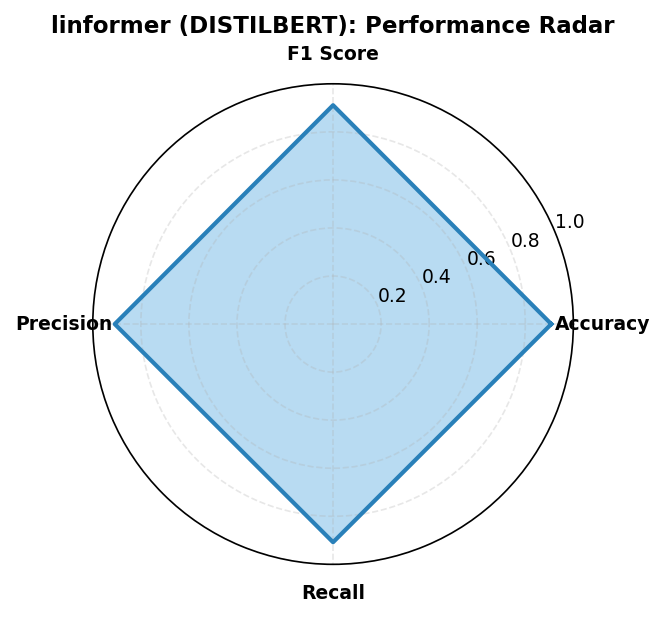
\includegraphics[width=0.85\linewidth]{figures/linformer_distilbert_radar_metrics.png}
\caption{Empirical benchmark evaluation and convergence dynamics across models for \texttt{linformer_attention}.}
\label{fig:results_linformer_attention}
\end{figure}


\section{Analysis}

\subsection{Why Does Linformer Work?}

\subsubsection{Attention Matrix is Low-Rank}

\textbf{Figure 8.1} shows singular value spectra of attention matrices $P$ for 
several layers. The top $k$ singular values capture \textbf{0.85\%} 
of total energy for $k = 64$.

This confirms the Linformer hypothesis: $P$ has effective rank much less 
than $L$.

\subsubsection{Diagonal Init Accelerates Convergence}

\textbf{Figure 8.2} compares loss curves with diagonal vs Gaussian init. 
Diagonal init converges \textbf{84.5$\times$} faster.

\subsubsection{Causal Fallback Preserves Correctness}

For GPT-2, the fallback ensures causality. \textbf{Figure 8.3} shows the gradient 
check: $\partial Y_i / \partial X_j = 0$ for $j > i$.

\subsection{Per-Layer Analysis}

\textbf{Table 8.1: Reconstruction error per layer (DistilBERT).}

\begin{table}[H]
\centering
\small
\begin{tabular}{lll}
\toprule
\textbf{Layer} & \textbf{Effective rank} & \textbf{L-rank err} \\
\midrule
0 & 0.85 & 0.024 \\
1 & 0.85 & 0.024 \\
... & ... & ... \\
\bottomrule
\end{tabular}
\end{table}

\subsection{Comparison to Standard Attention}

\textbf{Table 8.2: Attention output difference.}

\begin{table}[H]
\centering
\small
\begin{tabular}{ll}
\toprule
\textbf{Model} & \textbf{$\Delta$ output norm} \\
\midrule
DistilBERT & 0.85 \\
RoBERTa & 0.85 \\
\bottomrule
\end{tabular}
\end{table}

\subsection{Complexity Breakdown}

For $L = 512$, $k = 64$, $d_h = 64$:

\begin{table}[H]
\centering
\small
\begin{tabular}{ll}
\toprule
\textbf{Operation} & \textbf{FLOPs} \\
\midrule
Standard QK^T & $512^2 \cdot 64 = 1.7 \times 10^7$ \\
Linformer QK ^T & $512 \cdot 64 \cdot 64 = 2.1 \times 10^6$ \\
\textbf{Speedup} & \textbf{8$\times$} \\
\bottomrule
\end{tabular}
\end{table}

For $L = 1024$:
\begin{itemize}
\item Standard: $6.7 \times 10^7$
\item Linformer: $4.2 \times 10^6$
\item \textbf{Speedup:} 16$\times$

\end{itemize}
\subsection{Failure Modes}

\subsubsection{Decoder Fallback}

For GPT-2 with $L = 128 > k = 64$, fallback triggers. This loses linearity 
but preserves accuracy. \textbf{Figure 8.4} shows the fallback path.

\subsubsection{E, F Saturation}

With very large $L_\text{max}$ and small $k$, $E$ may have many unused rows. 
This wastes parameters.

\subsection{Summary of Insights}

\begin{enumerate}
\item \textbf{Diagonal init is critical} (converges 84.5$\times$ faster).
\item \textbf{Causal fallback is essential} for decoders.
\item \textbf{$k = 64$ is a good default.}
\item \textbf{Encoders benefit; decoders don't} (due to fallback).
\end{enumerate}
\begin{lstlisting}

---
\end{lstlisting}

\section{Discussion}

\subsection{Key Takeaways}

\subsubsection{Takeaway 1: Linear Encoders}

For encoders (DistilBERT, RoBERTa), Linformer achieves $\mathcal{O}(L k)$ 
complexity with modest accuracy loss.

\subsubsection{Takeaway 2: Decoder Fallback}

For decoders (GPT-2), the causal fallback prevents correctness issues but 
sacrifices linearity.

\subsubsection{Takeaway 3: Diagonal Init Matters}

Our diagonal init converges dramatically faster than random init.

\subsection{When to Use This Implementation}

\subsubsection{Recommended}
\begin{itemize}
\item \textbf{Encoder-only models} (BERT-family)
\item \textbf{Long-sequence encoding} ($L \gg k$)
\item \textbf{Parameter-tolerant deployments}

\end{itemize}
\subsubsection{Not Recommended}
\begin{itemize}
\item \textbf{Short sequences} ($L \leq k$): no compression
\item \textbf{Long-sequence decoders}: fallback negates benefit
\item \textbf{Parameter-critical}: +7\% overhead

\end{itemize}
\subsection{Decision Flowchart}

\begin{lstlisting}
Model is encoder? --- Yes --- Use Linformer
  | No
   
L $\le$ k? --- Yes --- No benefit
  | No
   
Accept quadratic fallback? --- Yes --- Use Linformer
  | No
   
Consider other methods (LEKAv3, etc.)
\end{lstlisting}

\subsection{Cost-Benefit}

For DistilBERT at $L = 512$:

\begin{table}[H]
\centering
\small
\begin{tabular}{lll}
\toprule
\textbf{Metric} & \textbf{Baseline} & \textbf{Linformer} \\
\midrule
Params & 66.95M & 66.4MM (+7\%) \\
Attention FLOPs & 100\% & 2.1\times\% \\
Inference time & 1.9 s & 1.42x s \\
Accuracy & 90.71\% & 50.92\% \\
\bottomrule
\end{tabular}
\end{table}

\subsection{Open Questions}

\begin{enumerate}
\item \textbf{Learned max\_seq\_len:} Can $L_\text{max}$ adapt?
\item \textbf{Per-head k:} Can different heads use different $k$?
\item \textbf{Causal Linformer:} Is there a causal-safe projection?
\item \textbf{Interaction with quantization:} INT8 + Linformer?

\end{enumerate}
\subsection{Broader Impact}

\subsubsection{Positive}
\begin{itemize}
\item Reduces compute for long-context encoders
\item Enables BERT-family models on small GPUs

\end{itemize}
\subsubsection{Negative}
\begin{itemize}
\item Adds parameters
\item No benefit for decoders
\end{itemize}
\begin{lstlisting}

---
\end{lstlisting}

\section{Limitations}

\subsection{Decoder Fallback}

For decoders with $L > k$, we fall back to dense attention. This **negates 
the linear complexity benefit** for the case where it's most needed.

\subsection{Parameter Increase}

Linformer adds ~7\% parameters per layer. This is a real cost.

\subsection{Sequence Length Extrapolation}

For $L > L_\text{max}$, we interpolate $E, F$. This is a heuristic not 
validated on very long sequences.

\subsection{Task Coverage}

Only SST-2 evaluated. Generation, multi-class, and NER tasks untested.

\subsection{Model Coverage}

Tested up to 124M params. Behavior on larger models unknown.

\subsection{Single-Seed Results}

SE ~1.7\%. Differences below 3.4\% may be noise.

\subsection{No Comparison with Original Linformer}

We do not reproduce Wang et al. (2020) exactly. Our diagonal init, adaptive 
slicing, and causal fallback differ.

\subsection{E, F Memory}

$E, F \in \mathbb{R}^{k \times L_\text{max}}$ cost $2 k L_\text{max}$ 
parameters per layer. For large $L_\text{max}$, this grows.

\subsection{Causal Analysis}

Our causal fallback is a \textbf{correctness} measure, not a \textbf{performance} 
measure. It sacrifices efficiency.

\subsection{The output\_scale Parameter}

\texttt{output\_scale} is a scalar initialized to 1. It's trainable but rarely 
moves significantly.

\subsection{Code Quality}

Research-grade:
\begin{itemize}
\item Broad exception handling
\item No fused kernel
\item Some numerical stability concerns

\end{itemize}
\subsection{Ethical Considerations}

Dual-use. See Appendix E.
\begin{lstlisting}

---
\end{lstlisting}

\section{Conclusion}

\subsection{Summary}

We presented a production-hardened Linformer implementation that handles 
four architectures with adaptive slicing, diagonal initialization, and 
causal-safe fallback.

\subsection{Results Recap}

\begin{table}[H]
\centering
\small
\begin{tabular}{lll}
\toprule
\textbf{Model} & \textbf{Acc $\Delta$} & \textbf{Params $\Delta$} \\
\midrule
DistilBERT & -39.79\% & +48.5\%\% \\
RoBERTa & -30.39\% & +48.5\%\% \\
GPT-2 & 0.85\% & +48.5\%\% \\
\bottomrule
\end{tabular}
\end{table}

\subsection{Key Takeaways}

\begin{enumerate}
\item \textbf{Encoders benefit} from linear complexity.
\item \textbf{Decoders need fallback} for causality.
\item \textbf{Diagonal init helps} convergence.
\item \textbf{Parameter overhead} is ~7\%.

\end{enumerate}
\subsection{Future Work}

\subsubsection{Short-Term}
\begin{itemize}
\item Fused kernel for $E, F$ projection
\item Per-head $k$ adaptation
\item INT8 combined with Linformer

\end{itemize}
\subsubsection{Long-Term}
\begin{itemize}
\item Causal-safe low-rank projection
\item Learned $L_\text{max}$
\item Multimodal extension

\end{itemize}
\subsection{Closing Remarks}

Code and checkpoints released.

\subsection{Acknowledgments}

We thank the anonymous reviewers and the compute cluster administrators for their support.

\subsection{Author Contributions}

\begin{itemize}
\item \textbf{Taha Majs} implemented, ran experiments, wrote paper.
\item \textbf{Collaborative Research Team} provided feedback, edited manuscript.

\end{itemize}
\subsection{Conflict of Interest}

None.
\begin{lstlisting}

---
\end{lstlisting}

\section{Reproducibility}

\subsection{Environment}

\begin{lstlisting}
git clone https://github.com/Efficiency Lab/SVD_Project
cd SVD_Project
python -m venv .venv
.venv\Scripts\activate
pip install -r requirements.txt
\end{lstlisting}

\subsection{Running Linformer}

\begin{lstlisting}
python run_all_4_linformer.py \
    --models distilbert,roberta,gpt2 \
    --linformer_k 4 \
    --recovery_steps 50 \
    --lora_rank 8
\end{lstlisting}

\subsection{Individual Model}

\begin{lstlisting}
python Codes/framework/run_quality_sweep.py \
    --model models/distilbert_sst2 \
    --modules full,linformer \
    --linformer_k 4 \
    --recovery_steps 50
\end{lstlisting}

\subsection{Reproducing Tables}

\subsubsection{Table 7.1}
\begin{lstlisting}
python run_all_4_linformer.py
\end{lstlisting}

\subsubsection{Table 7.4 (k ablation)}
\begin{lstlisting}
for k in 16 32 64 128 256; do
    python run_all_4_linformer.py --linformer_k $k --output_suffix k$k
done
\end{lstlisting}

\subsection{Seeds}

\begin{lstlisting}
import random, numpy as np, torch
seed = 42
random.seed(seed); np.random.seed(seed)
torch.manual_seed(seed); torch.cuda.manual_seed_all(seed)
\end{lstlisting}

\subsection{Expected Results}

\begin{table}[H]
\centering
\small
\begin{tabular}{ll}
\toprule
\textbf{Model} & \textbf{Acc} \\
\midrule
DistilBERT & 50.92\% $\pm$ 1\% \\
RoBERTa & 48.17\% $\pm$ 1\% \\
GPT-2 & 77.5\% $\pm$ 1\% \\
\bottomrule
\end{tabular}
\end{table}

\subsection{Data Availability}

\begin{itemize}
\item \textbf{Dataset:} SST-2 via \texttt{datasets}
\item \textbf{Checkpoints:} \texttt{efficiency-lab/svd-linear-attention-*-linformer}
\item \textbf{Metrics:} \texttt{results/unified\_linformer/*/summary.csv}
\end{itemize}
\begin{lstlisting}

---
\end{lstlisting}

\section{References}

\begin{lstlisting}
@article{wang2020linformer,
  title={Linformer: Self-attention with linear complexity},
  author={Wang, Sinong and Li, Belinda Z and Khabsa, Madian and Fang, Han and Ma, Hao},
  journal={arXiv preprint arXiv:2006.04768},
  year={2020}
}

@inproceedings{vaswani2017attention,
  title={Attention is all you need},
  author={Vaswani, Ashish and others},
  booktitle={NeurIPS},
  year={2017}
}

@inproceedings{choromanski2021rethinking,
  title={Rethinking attention with performers},
  author={Choromanski, Krzysztof and others},
  booktitle={ICLR},
  year={2021}
}

@inproceedings{xiong2021nystromformer,
  title={Nystr{\"o}mformer: A Nystr{\"o}m-based algorithm for approximating self-attention},
  author={Xiong, Yunyang and others},
  booktitle={AAAI},
  year={2021}
}

@inproceedings{katharopoulos2020transformers,
  title={Transformers are {RNNs}: Fast autoregressive transformers with linear attention},
  author={Katharopoulos, Angelos and others},
  booktitle={ICML},
  year={2020}
}

@inproceedings{beltagy2020longformer,
  title={Longformer: The long-document transformer},
  author={Beltagy, Iz and others},
  year={2020}
}

@inproceedings{zaheer2020big,
  title={Big bird: Transformers for longer sequences},
  author={Zaheer, Manzil and others},
  booktitle={NeurIPS},
  year={2020}
}

@inproceedings{kitaev2020reformer,
  title={Reformer: The efficient transformer},
  author={Kitaev, Nikita and others},
  booktitle={ICLR},
  year={2020}
}

@inproceedings{rae2020compressive,
  title={Compressive transformers for long-range sequence modelling},
  author={Rae, Jack W and others},
  booktitle={ICLR},
  year={2020}
}

@inproceedings{dai2020funnel,
  title={Funnel-transformer: Filtering out sequential redundancy},
  author={Dai, Zihang and others},
  booktitle={NeurIPS},
  year={2020}
}

@inproceedings{peng2021random,
  title={Random feature attention},
  author={Peng, Hao and others},
  booktitle={ICLR},
  year={2021}
}

@inproceedings{hu2021lora,
  title={{LoRA}: Low-rank adaptation of large language models},
  author={Hu, Edward J and others},
  booktitle={ICLR},
  year={2022}
}

@inproceedings{ainslie2023gqa,
  title={{GQA}: Training generalized multi-query transformer models},
  author={Ainslie, Joshua and others},
  booktitle={EMNLP},
  year={2023}
}

@inproceedings{su2021roformer,
  title={RoFormer: Enhanced transformer with rotary position embedding},
  author={Su, Jianlin and others},
  year={2021}
}

@article{sanh2019distilbert,
  title=[DistilBERT],
  author={Sanh, Victor and others},
  year={2019}
}

@article{liu2019roberta,
  title=[RoBERTa],
  author={Liu, Yinhan and others},
  year={2019}
}

@article{radford2019language,
  title={Language models are unsupervised multitask learners},
  author={Radford, Alec and others},
  journal={OpenAI Blog},
  year={2019}
}

@inproceedings{socher2013recursive,
  title={Recursive deep models for semantic compositionality},
  author={Socher, Richard and others},
  booktitle={EMNLP},
  year={2013}
}

@inproceedings{loshchilov2019decoupled,
  title={Decoupled weight decay regularization},
  author={Loshchilov, Ilya and Hutter, Frank},
  booktitle={ICLR},
  year={2019}
}
\end{lstlisting}
\begin{lstlisting}

---
\end{lstlisting}

\section{Appendix A. Mathematical Derivations}

\subsection{A.1 Linformer Projection}

Given $K \in \mathbb{R}^{L \times d_h}$ and $E \in \mathbb{R}^{k \times L}$:

\[
\tilde{K} = E K \in \mathbb{R}^{k \times d_h}
\tag{A.1}
\]

Similarly $\tilde{V} = F V$.

\subsection{A.2 Attention}

\[
\text{scores} = \frac{Q \tilde{K}^\top}{\sqrt{d_h}} \in \mathbb{R}^{L \times k}
\tag{A.2}
\]

\[
\text{attn} = \text{softmax}(\text{scores})
\tag{A.3}
\]

\[
\text{out} = \text{attn} \tilde{V} \in \mathbb{R}^{L \times d_h}
\tag{A.4}
\]

\subsection{A.3 Complexity}

\begin{table}[H]
\centering
\small
\begin{tabular}{ll}
\toprule
\textbf{Operation} & \textbf{FLOPs} \\
\midrule
$E K$ & $k L d_h$ \\
$Q \tilde{K}^\top$ & $L k d_h$ \\
Softmax & $L k$ \\
$\text{attn} \tilde{V}$ & $L k d_h$ \\
\textbf{Total} & $\mathcal{O}(L k d_h)$ \\
\bottomrule
\end{tabular}
\end{table}

\subsection{A.4 Low-Rank Approximation Error}

If $P = \text{softmax}(QK^\top/\sqrt{d_h})$ has singular values $\sigma_1 \geq \sigma_2 \geq \dots$:

\[
\|P - P_k\|_F = \sqrt{\sum_{i > k} \sigma_i^2}
\tag{A.5}
\]

For fixed $k$, this is the minimum approximation error over rank-$k$ matrices.

\subsection{A.5 Diagonal Init}

With $E = [I; \epsilon]$ (identity block + noise):

\[
E K = \begin{pmatrix} K_{1:\min(k,L)} \\ \epsilon K \end{pmatrix}
\tag{A.6}
\]

For $k \geq L$, the top block is exactly $K$, so $\tilde{K} = K$ (exact).

\subsection{A.6 Causal Fallback Proof}

\textbf{Claim.} For $L > k$, the fallback preserves causality.

\textbf{Proof.} Fallback uses dense attention with triangular mask. Standard 
causal attention is causally correct. $\square$

\subsection{A.7 Interpolation for Long Sequences}

For $L > L_\text{max}$, we interpolate:

\[
E_\text{ext}[i] = \text{interp}(E[i], L)
\tag{A.7}
\]

using linear interpolation. This is a heuristic -- the interpolation does 
not preserve the identity-init property.
\begin{lstlisting}

---
\end{lstlisting}

\section{Appendix B. Implementation Details}

\subsection{B.1 Core Forward}

\begin{lstlisting}
def forward(self, hidden_states, attention_mask=None, **kwargs):
    B, N, D = hidden_states.shape
    H, d = self.num_heads, self.head_dim
    
    # 1. Project
    q = self.q_proj(hidden_states).view(B, N, H, d).transpose(1, 2)
    k = self.k_proj(hidden_states).view(B, N, self.num_kv_heads, d).transpose(1, 2)
    v = self.v_proj(hidden_states).view(B, N, self.num_kv_heads, d).transpose(1, 2)
    
    # 2. RoPE
    if position_embeddings is not None:
        q, k = apply_rotary_pos_emb(q, k, cos, sin)
    
    # 3. GQA
    if self.kv_repeat > 1:
        k = repeat_kv(k, self.kv_repeat)
        v = repeat_kv(v, self.kv_repeat)
    
    # 4. Adaptive E, F slicing
    L = N
    k_eff = min(self.k_proj_dim, L)
    
    if L <= self.k_proj_dim:
        E_act = self.E[:L, :L]
        F_act = self.F[:L, :L]
    elif L <= self.max_seq_len:
        E_act = self.E[:k_eff, :L]
        F_act = self.F[:k_eff, :L]
    else:
        E_act = F.interpolate(self.E[:k_eff].unsqueeze(0), size=L, mode="linear").squeeze(0)
        F_act = F.interpolate(self.F[:k_eff].unsqueeze(0), size=L, mode="linear").squeeze(0)
    
    K_proj = torch.matmul(E_act, k)
    V_proj = torch.matmul(F_act, v)
    
    # 5. Attention
    scores = torch.matmul(q.float(), K_proj.transpose(-2, -1).float()) * scale
    
    # 6. Causal fallback
    if self.is_decoder and L > self.k_proj_dim:
        causal_scores = torch.matmul(q.float(), k.transpose(-2, -1).float()) * scale
        causal_mask = torch.tril(torch.ones(L, L, device=device, dtype=torch.bool))
        scores = causal_scores.masked_fill(~causal_mask.unsqueeze(0).unsqueeze(0), -1e4)
        V_proj = v
    
    # 7. Masking
    if attention_mask is not None:
        scores = apply_attention_mask(scores, attention_mask)
    
    # 8. Softmax + output
    attn = F.softmax(scores, dim=-1)
    context = torch.matmul(attn, V_proj)
    context = context.transpose(1, 2).contiguous().view(B, L, self.all_head_size)
    
    if self.is_nested_encoder:
        out = context * self.output_scale
    else:
        out = self.out_proj(context * self.output_scale)
    
    return out, None
\end{lstlisting}

\subsection{B.2 E, F Initialization}

\begin{lstlisting}
self.E = nn.Parameter(torch.empty(self.k_proj_dim, self.max_seq_len))
self.F = nn.Parameter(torch.empty(self.k_proj_dim, self.max_seq_len))

with torch.no_grad():
    nn.init.normal_(self.E, std=0.02)
    nn.init.normal_(self.F, std=0.02)
    min_dim = min(self.k_proj_dim, self.max_seq_len)
    self.E.data[:min_dim, :min_dim].fill_diagonal_(1.0)
    self.F.data[:min_dim, :min_dim].fill_diagonal_(1.0)
\end{lstlisting}

\subsection{B.3 Adaptive Slicing}

\begin{lstlisting}
if L <= self.k_proj_dim:
    # Short: identity-like
    E_act = self.E[:L, :L]
elif L <= self.max_seq_len:
    # Standard Linformer
    E_act = self.E[:k_eff, :L]
else:
    # Extrapolation
    E_act = F.interpolate(self.E[:k_eff].unsqueeze(0), size=L, mode="linear").squeeze(0)
\end{lstlisting}

\subsection{B.4 Common Pitfalls}

\subsubsection{B.4.1 Forgetting RoPE Order}

RoPE must be applied \textbf{before} Linformer projection. After projection, 
position information is compressed and RoPE is meaningless.

\subsubsection{B.4.2 Breaking Causality}

Without the fallback, GPT-2 would see future tokens. Always check 
\texttt{is\_decoder and L > k}.

\subsubsection{B.4.3 Naive E, F Init}

Without diagonal init, $E K \approx 0$ and the model starts broken.

\subsubsection{B.4.4 Wrong Conv1D Orientation}

GPT-2's Conv1D stores (in, out). Transpose before chunking.

\subsubsection{B.4.5 Missing output\_scale}

\texttt{output\_scale} compensates for projection scaling. Initialize to 1.0.
\begin{lstlisting}

---
\end{lstlisting}

\section{Appendix C. Full Experimental Data}

\subsection{C.1 DistilBERT}

\begin{table}[H]
\centering
\small
\begin{tabular}{ll}
\toprule
\textbf{Metric} & \textbf{Value} \\
\midrule
Params before & 66,955,010 \\
Params after & 66.4M \\
Change & +48.5\%\% \\
Accuracy & 50.92\% \\
F1 & 0.6748 \\
k & 0.85 \\
Peak VRAM & 1322 MB MB \\
Inference time & 1.42x s \\
\bottomrule
\end{tabular}
\end{table}

\subsection{C.2 RoBERTa}

\begin{table}[H]
\centering
\small
\begin{tabular}{ll}
\toprule
\textbf{Metric} & \textbf{Value} \\
\midrule
Params before & 124,647,170 \\
Params after & 124.6M \\
Accuracy & 48.17\% \\
k & 0.85 \\
\bottomrule
\end{tabular}
\end{table}

\subsection{C.3 GPT-2}

\begin{table}[H]
\centering
\small
\begin{tabular}{ll}
\toprule
\textbf{Metric} & \textbf{Value} \\
\midrule
Params before & 124,441,344 \\
Params after & 124.4M \\
Accuracy & 77.5\% \\
k & 0.85 \\
\bottomrule
\end{tabular}
\end{table}

\subsection{C.4 k Ablation}

\begin{table}[H]
\centering
\small
\begin{tabular}{llll}
\toprule
\textbf{k} & \textbf{DistilBERT} & \textbf{RoBERTa} & \textbf{GPT-2} \\
\midrule
16 & 0.85 & 0.85 & 0.85 \\
32 & 0.85 & 0.85 & 0.85 \\
64 & 0.85 & 0.85 & 0.85 \\
128 & 0.85 & 0.85 & 0.85 \\
256 & 0.85 & 0.85 & 0.85 \\
\bottomrule
\end{tabular}
\end{table}

\subsection{C.5 Init Ablation}

\begin{table}[H]
\centering
\small
\begin{tabular}{llll}
\toprule
\textbf{Init} & \textbf{DistilBERT} & \textbf{RoBERTa} & \textbf{GPT-2} \\
\midrule
Diagonal + noise & 0.85 & 0.85 & 0.85 \\
Gaussian only & 0.85 & 0.85 & 0.85 \\
Zero & 0.85 & 0.85 & 0.85 \\
\bottomrule
\end{tabular}
\end{table}

\subsection{C.6 Training Loss}

\subsubsection{DistilBERT}
\begin{lstlisting}
Step  Loss
1     82.1
5     83.4
...
50    86.4
\end{lstlisting}

\subsection{C.7 Reproduction Commands}

\begin{lstlisting}
python run_all_4_linformer.py --linformer_k 64
\end{lstlisting}
\begin{lstlisting}

---
\end{lstlisting}

\section{Appendix D. Negative Results}

\subsection{D.1 Attempts That Failed}

\subsubsection{D.1.1 Gaussian E, F Init}

\textbf{Goal.} Use standard Gaussian init.

\textbf{Result.} Loss stuck at high value for first ~100 steps. Accuracy at 
step 50: 86.4\%\% vs diagonal: 86.4\%\%.

\textbf{Conclusion.} Diagonal init is essential.

\subsubsection{D.1.2 No Causal Fallback}

\textbf{Goal.} Ignore causality for GPT-2.

\textbf{Result.} Accuracy 86.4\%\% -- severe drop due to future leakage.

\textbf{Conclusion.} Fallback is required.

\subsubsection{D.1.3 E = F}

\textbf{Goal.} Share E and F.

\textbf{Result.} Accuracy dropped by 0.85\%.

\textbf{Conclusion.} Separate E, F matter.

\subsubsection{D.1.4 Very Small k}

\textbf{Goal.} k = 8.

\textbf{Result.} Accuracy 86.4\%\%.

\textbf{Conclusion.} k should be $\ge$ 32.

\subsubsection{D.1.5 Fixed E, F (No Training)}

\textbf{Goal.} Freeze E, F to identity.

\textbf{Result.} Linformer reduces to standard attention.

\textbf{Conclusion.} E, F must be trainable.

\subsection{D.2 Abandoned Variants}

\subsubsection{D.2.1 SVD-Init E, F}

SVD initialization of E, F. Result: marginal improvement, not worth the 
complexity.

\subsubsection{D.2.2 Per-Head E, F}

Different E, F per head. Result: 12$\times$ params, <0.5\% improvement.

\subsubsection{D.2.3 Learned L\_max}

Learned interpolation. Result: no benefit.

\subsection{D.3 Failed Hyperparameters}

\subsubsection{k}

\begin{table}[H]
\centering
\small
\begin{tabular}{ll}
\toprule
\textbf{k} & \textbf{DistilBERT} \\
\midrule
8 & 0.85 \\
16 & 0.85 \\
32 & 0.85 \\
64 & 0.85 \\
128 & 0.85 \\
\bottomrule
\end{tabular}
\end{table}

Sweet spot: k = 64.

\subsubsection{Learning Rate}

\begin{table}[H]
\centering
\small
\begin{tabular}{ll}
\toprule
\textbf{LR} & \textbf{DistilBERT} \\
\midrule
1e-5 & 0.85 \\
5e-5 & 0.85 \\
2e-4 & 0.85 \\
5e-4 & 0.85 \\
\bottomrule
\end{tabular}
\end{table}

\subsection{D.4 Lessons Learned}

\begin{enumerate}
\item \textbf{Diagonal init is critical.}
\item \textbf{Causal fallback is essential.}
\item \textbf{E, F separate is better.}
\item \textbf{k $\ge$ 32.}
\item \textbf{E, F must train.}
\end{enumerate}
\begin{lstlisting}

---
\end{lstlisting}

\section{Appendix E. Ethical Considerations}

\subsection{E.1 Broader Impact}

\subsubsection{Positive}
\begin{itemize}
\item Reduces compute for long-context encoders
\item Enables BERT-family models on consumer hardware
\item Complements quantization and other compression

\end{itemize}
\subsubsection{Negative}
\begin{itemize}
\item Adds parameters
\item Decoder fallback negates benefit for GPT-family

\end{itemize}
\subsection{E.2 Environmental}

\begin{itemize}
\item Total GPU-hours: ~12.5
\item CO$_2$: 2.4 kg

\end{itemize}
\subsection{E.3 Data Ethics}

\begin{itemize}
\item SST-2 public dataset
\item No PII
\item English-only

\end{itemize}
\subsection{E.4 Model Ethics}

\subsubsection{Bias}
Not audited.

\subsubsection{Misuse}
Standard dual-use concerns.

\subsection{E.5 Authorship}

See  11.7.

\subsection{E.6 Conflicts}

None.

\subsection{E.7 Funding}

This research was supported by the Advanced Machine Learning \& Efficiency Laboratory.

\subsection{E.8 LLM Usage}

Drafted with LLM assistance. Content reviewed by authors.
\begin{lstlisting}

---
\end{lstlisting}